\chapter{MULTI-PORT RAM}
\label{chp:memory}
The repeated values array requires a large amount of space. To efficiently store this array on the FPGA we created a shared memory. It is a component in the larger design for a sparse matrix vector multiplier. Specifically it allows the decoder to access more memory space without going off chip. The component allows each PE to access a table that is 16 times larger than if it was stored inside each PE. Multi-port RAMs have been designed before, but none achieve our desired performance.

\section{Related Work}
\label{sec:relatedwork}
FPGAs have RAM blocks for designs that require large amounts of memory space. Four strategies exist for creating multi-port memory with RAM blocks: {\em multi-pumping}, {\em replication}, {\em Live Value Table}, and {\em banking}. \par
{\em Multi-pumping}, seen in \cite{prelim:manjikian,prelim:canis,prelim:yantir}, cannot support our desired clock frequency. {\em Replication}, seen in \cite{prelim:fort,prelim:mousali,prelim:yiannacouras}, and {\em Live Value Table}, seen in \cite{prelim:laforest,prelim:anjam,prelim:abdelhadi}, store excessive redundant information information in RAM blocks. This leaves {\em Banking}, seen in \cite{prelim:moscola,prelim:saghir,prelim:saghir2}, which can scale to 16 or more ports.\par

    \begin{figure}
        \center
        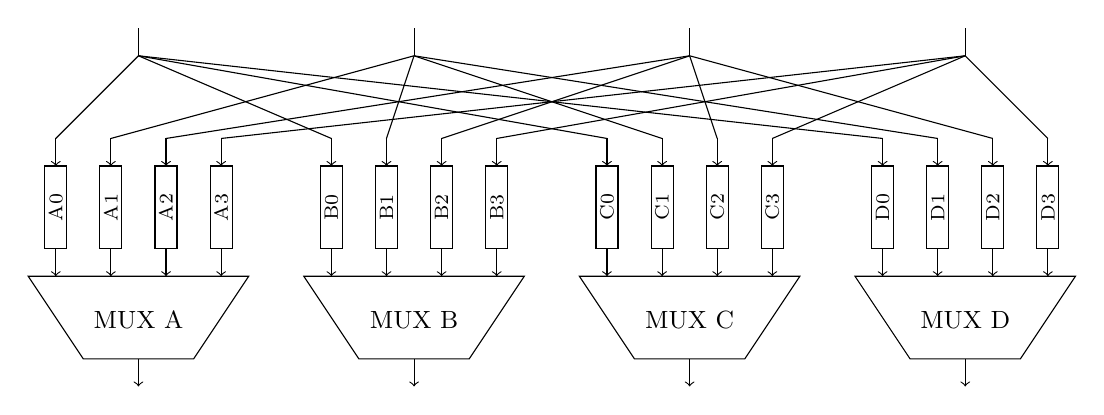
\begin{tikzpicture}[scale=.7]
            \foreach \i/\l in {0/A, 5/B, 10/C, 15/D}{
                \draw[xshift=\i cm] (-2,1) -- (2,1) -- (1,-.5) -- (-1,-.5) -- cycle;
                \node at (\i,.2){\small MUX \l};
                \draw [xshift=\i cm,->](0,-.5) -- (0,-1);
                \foreach \j/\p in {-1.5/0, -.5/1, .5/2,1.5/3}{
                    \draw [xshift = \i cm](\j-.2,1.5) rectangle (\j+.2,3);
                    \node at (\i+\j,2.25)[rotate=90]{\scriptsize \l\p};
                    \draw [xshift = \i cm,->](\j,1.5) -- (\j,1);
                    \draw [xshift = \i cm,->](\j,3.5) -- (\j,3);
                }
            }
            \foreach \i/\j in {0/-1.5, 5/-.5, 10/.5, 15/1.5}{
                \foreach \k in {0, 5, 10, 15}{
                    \draw (\i, 5) -- (\k+\j, 3.5);
                }
                \draw (\i,5) -- (\i, 5.5);
            }
        \end{tikzpicture}
        \caption{The fully-connected interconnect network.}
        \label{fig:crossbar}
    \end{figure}

    A straight forward way to create this memory would use full-connected interconnect networks (\figurename~\ref{fig:crossbar}). Unfortunately, as the size of a fully-connected interconnect network grows, the more space the FIFOs and multiplexers require. A 8-to-1 multiplexer requires approximately twice the number of resources of a 4-to-1 multiplexer. This means the area the multiplexers require grows by around $N^2$. The number of FIFOs grows by $N^2$ as well.

\section{Omega Multi-port Memory}
    \begin{figure}
        \center
        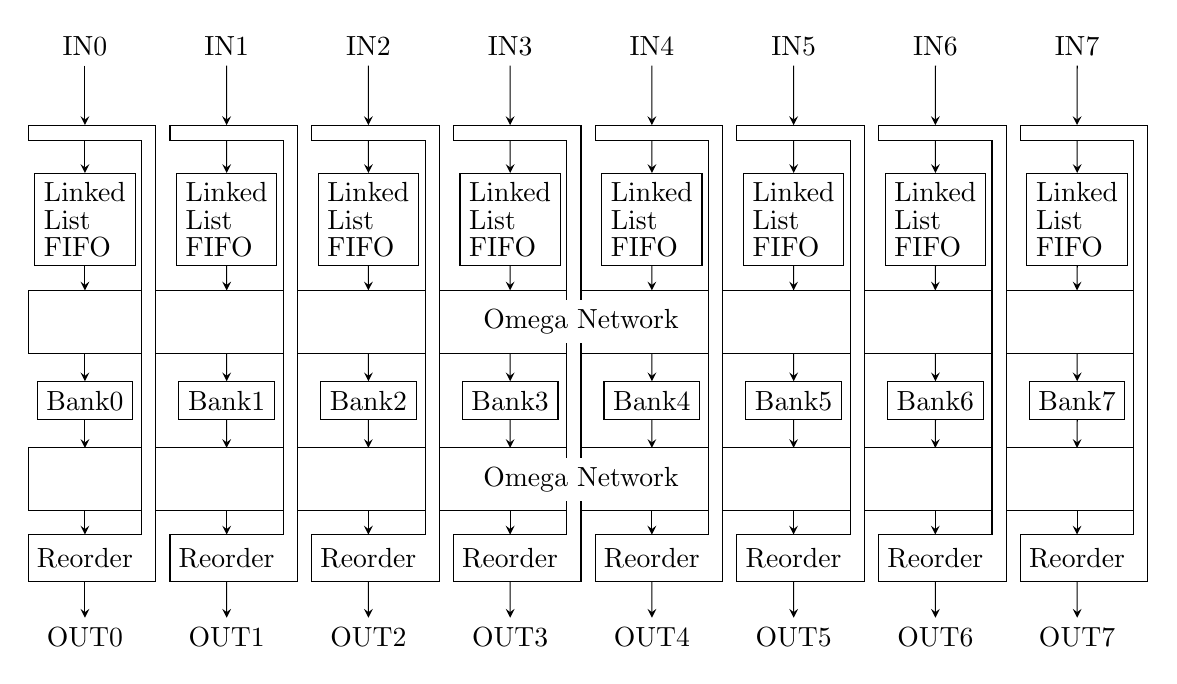
\begin{tikzpicture}[xscale=1.8]
            \draw (-.4,-1.6) rectangle (7.4,-2.4);
            \draw (-.4,-3.6) rectangle (7.4,-4.4);
            %\draw[dashed] (-.5,0) rectangle (3.5,-4.5);
            \foreach \x in {0,1,...,7}{
                \node at (\x,1.5)(in){IN\x};
                \node at (\x,-6)(out){OUT\x};
                \draw[xshift=\x cm - .1 cm,fill=white](-.3,.5) -- (-.3,.3) -- (.5,.3) -- (.5,-4.7) -- (-.3,-4.7) -- (-.3,-5.3) -- (.6,-5.3) -- (.6, .5) -- cycle;
                \node at (\x, -5){Reorder};
                \node[draw] at (\x,-.7)(inBuf){\shortstack[l]{Linked\\List\\FIFO}};
                \node[draw] at (\x,-3)(mem){Bank\x};
                \path[draw,>=stealth,->] (in) -- (\x,.5);
                \path[draw,>=stealth,->] (\x,.3) -- (inBuf);
                \path[draw,>=stealth,->] (inBuf) -- (\x,-1.6);
                \path[draw,>=stealth,->] (\x,-2.4) -- (mem);
                \path[draw,>=stealth,->] (mem) -- (\x,-3.6);
                \path[draw,>=stealth,->] (\x,-4.4) -- (\x,-4.7);
                \path[draw,>=stealth,->] (\x,-5.3) -- (out);
            }
            \node[fill=white] at (3.5,-2){Omega Network};
            \node[fill=white] at (3.5,-4){Omega Network};
            %\node[xshift=-3,rotate=90,fill=white] at (-.5,-2){Multi-port Memory};

        \end{tikzpicture}
        \caption[The Omega multi-port memory.]{In the Omega multi-port memory all the buffering occurs in the linked list FIFOs. The use of multi-stage interconnect networks, in this case Omega networks, helps reduce the area of the design.}
        \label{fig:versionb}
    \end{figure}
    The Omega multi-port memory (\figurename~\ref{fig:versionb}) has hardware structures designed for scaling. Instead of using fully connected interconnect networks, area efficient multi-stage interconnect networks (MIN) route signals to and from the memory banks. In addition, this memory uses $N$ linked list FIFOs to buffer incoming requests, instead of $N^2$ FIFOs. These two structures pair well, because they both save logic resources. However, both share a common restriction; neither structure can simultaneously send multiple buffered messages, from the same port, to different banks.\par
    The Omega memory has several subcomponents: first, the memory banks for storing the data, second, Omega networks for routing between the ports and banks, third, linked list FIFOs to buffer requests to banks, fourth, reorder queues to reorder read responses.
\subsection{Memory Banks}
For any banking approach, a memory with $N$ ports requires at least $N$ RAM blocks. Each RAM block holds a unique segment of the total memory space. We have multiple options to decide how to segment the memory space. The simplest option assigns the first $N^{th}$ of the address space to Bank0, the next $N^{th}$ to Bank1, and so on. However, this approach can easily cause bottlenecks. For example, assume all the processing elements start to read from a low address located in Bank0 and continue to sequentially increment the read addresses. All the requests would route to Bank0, necessitating multiple stalls. The interleaving memory address space that our design uses decreases the chance these specific types of bottlenecks occur.
\subsection{Omega Network}
%    \begin{figure}
%        \center
%        \begin{subfigure}{.32\linewidth}
%        \center
%        \input{fig/banyan1.tex}
%        \caption{Banyan Switch}
%        \label{fig:banyan}
%    \end{subfigure}
%        \begin{subfigure}{.32\linewidth}
%        \center
%        \input{fig/banyanon.tex}
%        \caption{Banyan Switch in the on state}
%        \label{fig:banyanon}
%    \end{subfigure}
%        \begin{subfigure}{.32\linewidth}
%        \center
%        \input{fig/banyanoff.tex}
%        \caption{Banyan Switch in the off state}
%        \label{fig:banyanoff}
%    \end{subfigure}
%    \caption{}
%    \end{figure}
    \begin{figure}
        \center

        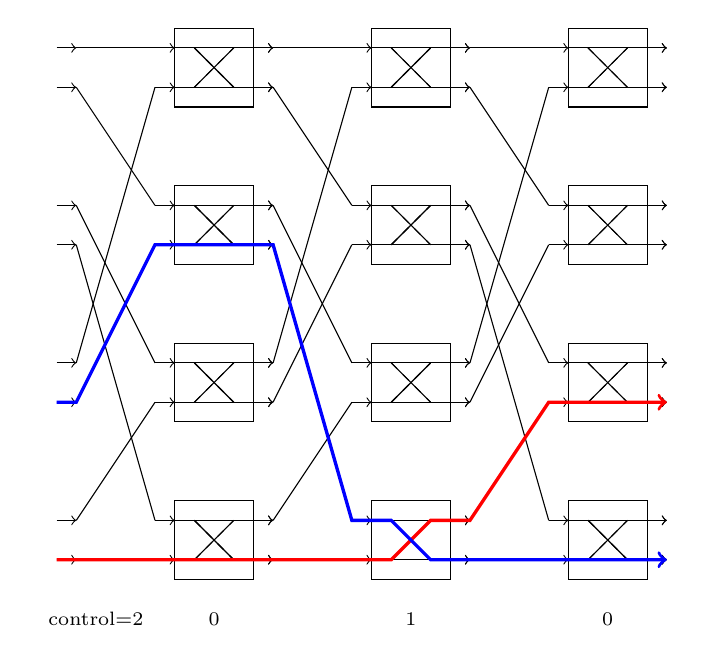
\begin{tikzpicture}[scale = .5]
            \foreach \i/\on in {0/0, 5/1, 10/0}{
                \foreach \j in {0, 4, 8, 12}{
                    \draw [shift={(\i,\j)}](-1,-1) rectangle (1,1);
                    \draw [shift={(\i,\j)}][->] (-1.5,-.5) -- (-1,-.5);
                    \draw [shift={(\i,\j)}][->] (-1.5,.5) -- (-1,.5);
                    \ifthenelse{\on=1}{
                        \draw [shift={(\i,\j)}](-.5,-.5) -- (.5,.5);
                        \draw [shift={(\i,\j)}](-.5,.5) -- (.5,-.5);
                        \draw [shift={(\i,\j)}] (-1,-.5) -- (-.5,-.5);
                        \draw [shift={(\i,\j)}] (-1,.5) -- (-.5,.5);
                        \draw [shift={(\i,\j)}][->] (.5,-.5) -- (1.5,-.5);
                        \draw [shift={(\i,\j)}][->] (.5,.5) -- (1.5,.5);
                        \draw [dashed,shift={(\i,\j)}](-.5,-.5) -- (.5,-.5);
                        \draw [dashed,shift={(\i,\j)}](-.5,.5) -- (.5,.5);
                    }{
                        \draw [shift={(\i,\j)}][->] (-1,-.5) -- (1.5,-.5);
                        \draw [shift={(\i,\j)}][->] (-1,.5) -- (1.5,.5);
                        \draw [dashed,shift={(\i,\j)}](-.5,-.5) -- (.5,.5);
                        \draw [dashed,shift={(\i,\j)}](-.5,.5) -- (.5,-.5);
                    }
                }
                \foreach \j/\k in {-.5/-.5,.5/3.5, 3.5/7.5, 4.5/11.5}{
                    \draw (\i-3.5, \j) -- (\i-1.5, \k);
                }
                \foreach \j/\k in {7.5/.5,8.5/4.5, 11.5/8.5, 12.5/12.5}{
                    \draw (\i-3.5, \j) -- (\i-1.5, \k);
                }
            }
            \foreach \i in {-.5,.5, 3.5,4.5, 7.5,8.5, 11.5,12.5}{
                \draw [->](-4,\i) -- (-3.5,\i);
            }
            \path[draw,red,very thick,->] (-4,-.5) -- (4.5,-.5) -- ++(1,1) -- ++(1,0) -- ++(2,3) -- ++(3,0);
            \path[draw,blue,very thick,->] (-4,3.5) -- ++(.5,0) -- ++(2,4) -- ++(3,0) -- ++(2,-7) -- ++(1,0) -- ++(1,-1) -- ++(6,0);
            \foreach [count=\c] \i in {-.5,.5, 3.5,4.5, 7.5,8.5, 11.5,12.5}{
                \FPeval{\z}{round(\c-1:0)};
                \node at (-4.5,\i) {\scriptsize \z};
                \node at (12,\i) {\scriptsize \z};
            }
            \node at (0,-2) {\scriptsize 0};
            \node at (5,-2) {\scriptsize 1};
            \node at (10,-2) {\scriptsize 0};
            \node at (-3,-2) {\scriptsize control=2};
        \end{tikzpicture}
        \caption[The Omega network.]{An 8-by-8 Omega network. We turn columns on or off to rotate between different routing configurations.}
        \label{fig:omega010}
    \end{figure}

    An Omega network consists of columns of Banyan switches~\cite{prelim:wu,prelim:lawrie}. A Banyan switch synthesizes to two multiplexers. In the on state, the switch crosses data over to the opposite output port. As an illustrative example, the second column in \figurename~\ref{fig:omega010} only contains switches in the on state. In the off state, the switch passes data straight to the corresponding output port. The first and last columns in \figurename~\ref{fig:omega010} only contain switches in the off state.

The Omega network has features that make it attractive in a multi-port memory design. If we switch whole columns of Banyan switches on or off, we can easily determine where signals route by XORing the starting port index with the bits controlling the columns. For example, in \figurename~\ref{fig:omega010}, the control bits equal $010_2$ or 2 and input port 2 ($010_2$) routes to output port 0. Not coincidentally, the same configuration routes in reverse. Input port 0 routes to output port 2 and input port 2 routes to output port 0. This means the design can use identical control bits for both the receiving and sending Omega networks.

In the Omega multi-port memory design, the control for this network increments every clock cycle. As an example, input port 5 would connect to output port 5, then port 4, 7, 6, 1, etc., until it cycles around again. This means each input connects to each output an equal number of times.

\subsection{The Linked List FIFO}
\label{sec:linkedfifo}
    \begin{figure}
        \center
        \begin{subfigure}{.4\linewidth}
        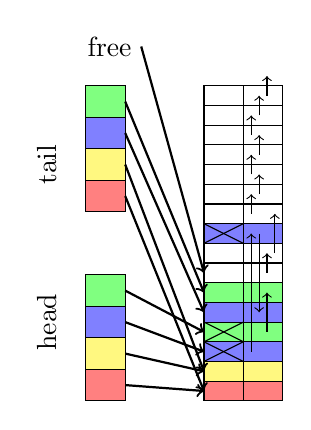
\begin{tikzpicture}
        \fill [red!50] (-.5,-2) rectangle (.5,-1.75);
        \fill [yellow!50] (-.5,-1.75) rectangle (.5,-1.5);
        \fill [blue!50] (-.5,-1.5) rectangle (.5,-1.25);
        \fill [blue!50] (-.5,-1) rectangle (.5,-.75);
        \fill [blue!50] (-.5,0) rectangle (.5,.25);
        \fill [green!50] (-.5,-1.25) rectangle (.5,-1);
        \fill [green!50] (-.5,-.5) rectangle (.5,-.75);
        \draw (-.5,-2) rectangle (0,2);
        \draw (0,-2) rectangle (.5,2);
        \foreach \i in {-1.75,-1.5,...,1.75}{
            \draw (-.5,\i) -- (.5,\i);
        }
        \node at (-2.5,-1)[rotate=90]{head};
        \node at (-2.5,1)[rotate=90]{tail};
        \node (f) at (-1.7,2.5) {free};
        \fill [red!50] (-2,-2) rectangle (-1.5,-1.6);
        \fill [yellow!50] (-2,-1.6) rectangle (-1.5,-1.2);
        \fill [blue!50] (-2,-1.2) rectangle (-1.5,-.8);
        \fill [green!50] (-2,-.8) rectangle (-1.5,-.4);
        \fill [red!50] (-2,.4) rectangle (-1.5,.8);
        \fill [yellow!50] (-2,.8) rectangle (-1.5,1.2);
        \fill [blue!50] (-2,1.2) rectangle (-1.5,1.6);
        \fill [green!50] (-2,1.6) rectangle (-1.5,2);
        \draw (-2,-2) rectangle (-1.5, -.4);
        \draw (-2,2) rectangle (-1.5, .4);
        \foreach \i in {-1.6,-1.2,-.8,.8,1.2,1.6}{
            \draw (-2,\i) -- (-1.5,\i);
        }
        \foreach[count=\i] \l/\h in {0/0,1/1,2/4,3/5}{
            \draw [thick,->] (-1.5,-1.8+\i*.4-.4) -- (-.5,\l*.25-1.875);
            \draw [thick,->] (-1.5,.6+\i*.4-.4) -- (-.5,\h*.25-1.875);
        }
        \draw (-.5,-1.5) -- (0,-1.25);
        \draw (-.5,-1.25) -- (0,-1.5);
        \draw (-.5,-1.25) -- (0,-1);
        \draw (-.5,-1) -- (0,-1.25);
        \draw (-.5,.25) -- (0,0);
        \draw (-.5,0) -- (0,.25);
        \draw [thick,->] (f.east) -- (-.5,-.375);
        \draw [->] (.1,-1.375) -- (.1,.125);
        \draw [->] (.2,.125) -- (.2,-.875);
        \draw [->] (.3,-.375) -- (.3,-.125);
        \draw [->] (.4,-.125) -- (.4,.375);
        \draw [->] (.3,-1.125) -- (.3,-.625);
        \foreach \i in {.375,.875,...,1.625}{
            \draw [->] (.1,\i) -- (.1,\i+.25);
            \draw [->] (.2,\i+.25) -- (.2,\i+.5);
        }
        \draw [->] (.3,1.875) -- (.3,2.125);

        \end{tikzpicture}
        \caption{Initial example}
        \label{fig:linked0}
    \end{subfigure}
        \begin{subfigure}{.4\linewidth}

        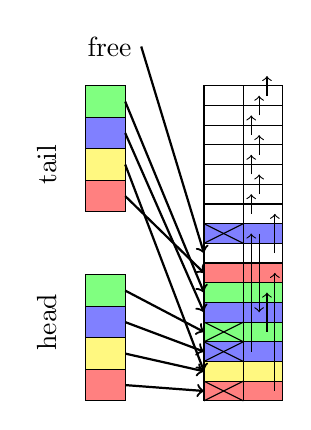
\begin{tikzpicture}
        \fill [red!50] (-.5,-2) rectangle (.5,-1.75);
        \fill [red!50] (-.5,-.5) rectangle (.5,-.25);
        \fill [yellow!50] (-.5,-1.75) rectangle (.5,-1.5);
        \fill [blue!50] (-.5,-1.5) rectangle (.5,-1.25);
        \fill [blue!50] (-.5,-1) rectangle (.5,-.75);
        \fill [blue!50] (-.5,0) rectangle (.5,.25);
        \fill [green!50] (-.5,-1.25) rectangle (.5,-1);
        \fill [green!50] (-.5,-.5) rectangle (.5,-.75);
        \draw (-.5,-2) rectangle (0,2);
        \draw (0,-2) rectangle (.5,2);
        \foreach \i in {-1.75,-1.5,...,1.75}{
            \draw (-.5,\i) -- (.5,\i);
        }
        \node at (-2.5,-1)[rotate=90]{head};
        \node at (-2.5,1)[rotate=90]{tail};
        \node (f) at (-1.7,2.5) {free};
        \fill [red!50] (-2,-2) rectangle (-1.5,-1.6);
        \fill [yellow!50] (-2,-1.6) rectangle (-1.5,-1.2);
        \fill [blue!50] (-2,-1.2) rectangle (-1.5,-.8);
        \fill [green!50] (-2,-.8) rectangle (-1.5,-.4);
        \fill [red!50] (-2,.4) rectangle (-1.5,.8);
        \fill [yellow!50] (-2,.8) rectangle (-1.5,1.2);
        \fill [blue!50] (-2,1.2) rectangle (-1.5,1.6);
        \fill [green!50] (-2,1.6) rectangle (-1.5,2);
        \draw (-2,-2) rectangle (-1.5, -.4);
        \draw (-2,2) rectangle (-1.5, .4);
        \foreach \i in {-1.6,-1.2,-.8,.8,1.2,1.6}{
            \draw (-2,\i) -- (-1.5,\i);
        }
        \foreach[count=\i] \l/\h in {0/6,1/1,2/4,3/5}{
            \draw [thick,->] (-1.5,-1.8+\i*.4-.4) -- (-.5,\l*.25-1.875);
            \draw [thick,->] (-1.5,.6+\i*.4-.4) -- (-.5,\h*.25-1.875);
        }
        \draw (-.5,-2) -- (0,-1.75);
        \draw (-.5,-1.75) -- (0,-2);
        \draw (-.5,-1.5) -- (0,-1.25);
        \draw (-.5,-1.25) -- (0,-1.5);
        \draw (-.5,-1.25) -- (0,-1);
        \draw (-.5,-1) -- (0,-1.25);
        \draw (-.5,.25) -- (0,0);
        \draw (-.5,0) -- (0,.25);
        \draw [thick,->] (f.east) -- (-.5,-.125);
        \draw [->] (.1,-1.375) -- (.1,.125);
        \draw [->] (.2,.125) -- (.2,-.875);
        \draw [->] (.4,-1.875) -- (.4,-.375);
        \draw [->] (.4,-.125) -- (.4,.375);
        \draw [->] (.3,-1.125) -- (.3,-.625);
        \foreach \i in {.375,.875,...,1.625}{
            \draw [->] (.1,\i) -- (.1,\i+.25);
            \draw [->] (.2,\i+.25) -- (.2,\i+.5);
        }
        \draw [->] (.3,1.875) -- (.3,2.125);

        \end{tikzpicture}
        \caption{First clock cycle}
        \label{fig:linked1}
    \end{subfigure}
        \begin{subfigure}{.4\linewidth}

        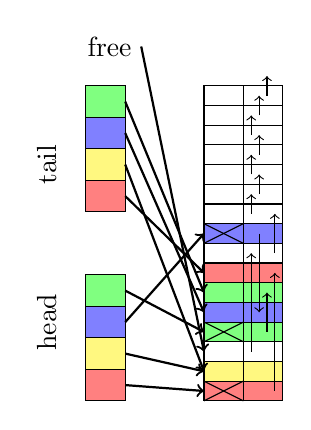
\begin{tikzpicture}
        \fill [red!50] (-.5,-2) rectangle (.5,-1.75);
        \fill [red!50] (-.5,-.5) rectangle (.5,-.25);
        \fill [yellow!50] (-.5,-1.75) rectangle (.5,-1.5);
        \fill [blue!50] (-.5,-1) rectangle (.5,-.75);
        \fill [blue!50] (-.5,0) rectangle (.5,.25);
        \fill [green!50] (-.5,-1.25) rectangle (.5,-1);
        \fill [green!50] (-.5,-.5) rectangle (.5,-.75);
        \draw (-.5,-2) rectangle (0,2);
        \draw (0,-2) rectangle (.5,2);
        \foreach \i in {-1.75,-1.5,...,1.75}{
            \draw (-.5,\i) -- (.5,\i);
        }
        \node at (-2.5,-1)[rotate=90]{head};
        \node at (-2.5,1)[rotate=90]{tail};
        \node (f) at (-1.7,2.5) {free};
        \fill [red!50] (-2,-2) rectangle (-1.5,-1.6);
        \fill [yellow!50] (-2,-1.6) rectangle (-1.5,-1.2);
        \fill [blue!50] (-2,-1.2) rectangle (-1.5,-.8);
        \fill [green!50] (-2,-.8) rectangle (-1.5,-.4);
        \fill [red!50] (-2,.4) rectangle (-1.5,.8);
        \fill [yellow!50] (-2,.8) rectangle (-1.5,1.2);
        \fill [blue!50] (-2,1.2) rectangle (-1.5,1.6);
        \fill [green!50] (-2,1.6) rectangle (-1.5,2);
        \draw (-2,-2) rectangle (-1.5, -.4);
        \draw (-2,2) rectangle (-1.5, .4);
        \foreach \i in {-1.6,-1.2,-.8,.8,1.2,1.6}{
            \draw (-2,\i) -- (-1.5,\i);
        }
        \foreach[count=\i] \l/\h in {0/6,1/1,8/4,3/5}{
            \draw [thick,->] (-1.5,-1.8+\i*.4-.4) -- (-.5,\l*.25-1.875);
            \draw [thick,->] (-1.5,.6+\i*.4-.4) -- (-.5,\h*.25-1.875);
        }
        \draw (-.5,-2) -- (0,-1.75);
        \draw (-.5,-1.75) -- (0,-2);
        \draw (-.5,-1.25) -- (0,-1);
        \draw (-.5,-1) -- (0,-1.25);
        \draw (-.5,.25) -- (0,0);
        \draw (-.5,0) -- (0,.25);
        \draw [thick,->] (f.east) -- (-.5,-1.375);
        \draw [->] (.1,-1.375) -- (.1,-.125);
        \draw [->] (.2,.125) -- (.2,-.875);
        \draw [->] (.4,-1.875) -- (.4,-.375);
        \draw [->] (.4,-.125) -- (.4,.375);
        \draw [->] (.3,-1.125) -- (.3,-.625);
        \foreach \i in {.375,.875,...,1.625}{
            \draw [->] (.1,\i) -- (.1,\i+.25);
            \draw [->] (.2,\i+.25) -- (.2,\i+.5);
        }
        \draw [->] (.3,1.875) -- (.3,2.125);

        \end{tikzpicture}
        \caption{Second clock cycle}
        \label{fig:linked2}
    \end{subfigure}
        \begin{subfigure}{.4\linewidth}
        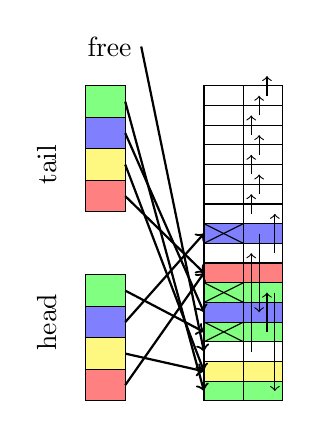
\begin{tikzpicture}
        \fill [green!50] (-.5,-2) rectangle (.5,-1.75);
        \fill [red!50] (-.5,-.5) rectangle (.5,-.25);
        \fill [yellow!50] (-.5,-1.75) rectangle (.5,-1.5);
        \fill [blue!50] (-.5,-1) rectangle (.5,-.75);
        \fill [blue!50] (-.5,0) rectangle (.5,.25);
        \fill [green!50] (-.5,-1.25) rectangle (.5,-1);
        \fill [green!50] (-.5,-.5) rectangle (.5,-.75);
        \draw (-.5,-2) rectangle (0,2);
        \draw (0,-2) rectangle (.5,2);
        \foreach \i in {-1.75,-1.5,...,1.75}{
            \draw (-.5,\i) -- (.5,\i);
        }
        \node at (-2.5,-1)[rotate=90]{head};
        \node at (-2.5,1)[rotate=90]{tail};
        \node (f) at (-1.7,2.5) {free};
        \fill [red!50] (-2,-2) rectangle (-1.5,-1.6);
        \fill [yellow!50] (-2,-1.6) rectangle (-1.5,-1.2);
        \fill [blue!50] (-2,-1.2) rectangle (-1.5,-.8);
        \fill [green!50] (-2,-.8) rectangle (-1.5,-.4);
        \fill [red!50] (-2,.4) rectangle (-1.5,.8);
        \fill [yellow!50] (-2,.8) rectangle (-1.5,1.2);
        \fill [blue!50] (-2,1.2) rectangle (-1.5,1.6);
        \fill [green!50] (-2,1.6) rectangle (-1.5,2);
        \draw (-2,-2) rectangle (-1.5, -.4);
        \draw (-2,2) rectangle (-1.5, .4);
        \foreach \i in {-1.6,-1.2,-.8,.8,1.2,1.6}{
            \draw (-2,\i) -- (-1.5,\i);
        }
        \foreach[count=\i] \l/\h in {6/6,1/1,8/4,3/0}{
            \draw [thick,->] (-1.5,-1.8+\i*.4-.4) -- (-.5,\l*.25-1.875);
            \draw [thick,->] (-1.5,.6+\i*.4-.4) -- (-.5,\h*.25-1.875);
        }
        \draw (-.5,-.75) -- (0,-.5);
        \draw (-.5,-.5) -- (0,-.75);
        \draw (-.5,-1.25) -- (0,-1);
        \draw (-.5,-1) -- (0,-1.25);
        \draw (-.5,.25) -- (0,0);
        \draw (-.5,0) -- (0,.25);
        \draw [thick,->] (f.east) -- (-.5,-1.375);
        \draw [->] (.1,-1.375) -- (.1,-.125);
        \draw [->] (.2,.125) -- (.2,-.875);
        \draw [->] (.4,-.625) -- (.4,-1.875);
        \draw [->] (.4,-.125) -- (.4,.375);
        \draw [->] (.3,-1.125) -- (.3,-.625);
        \foreach \i in {.375,.875,...,1.625}{
            \draw [->] (.1,\i) -- (.1,\i+.25);
            \draw [->] (.2,\i+.25) -- (.2,\i+.5);
        }
        \draw [->] (.3,1.875) -- (.3,2.125);

        \end{tikzpicture}
        \caption{Third clock cycle}
        \label{fig:linked3}
    \end{subfigure}
    \caption[The linked list FIFO.]{A linked list FIFO during 3 clock cycles of operation}
        \label{fig:linkedfifo}
    \end{figure}
    The partnering hardware structure, the linked list FIFO (\figurename~\ref{fig:linkedfifo}), contains several internal FIFOs with no predefined space in a single RAM. Similar to a software linked list, there exists a free pointer that points to the beginning of the free space linked list. Other variants of hardware linked list FIFOs exist [\cite{prelim:bell2,prelim:nikologiannis}].

    Due to the linking pointers, the size of the RAM now needs $O(N\log N)$ space to store $N$ elements. However $\log N$ grows slowly. For example, data stored in a 64-bit wide by 1024 deep RAM would need an additional 11-bit wide by 1024 deep RAM for the linking pointers. An illustrative example of the linked list FIFO is shown in in \figurename~\ref{fig:linkedfifo}, which uses a 16 deep RAM and 4 FIFOs.

    In the initial state (\figurename~\ref{fig:linked0}), the red and yellow FIFOs have no messages. The blue FIFO has two messages. And, the green FIFO has one message. However, every FIFO reserves one space for the next incoming value. This limits the total available space in the linked list FIFO to $TOTAL\_DEPTH-FIFO\_COUNT$.

         On the first clock cycle (\figurename~\ref{fig:linked1}), the linked list FIFO receives a push containing a red message. The new red message gets stored in the reserved space at the tail of the red linked list. The free linked list pops one space. That space gets pushed on to the red linked list.

         On the second clock cycle (\figurename~\ref{fig:linked2}), the linked list FIFO receives a pop for a blue message. A blue message gets popped from the head of the blue linked list. The newly freed space gets pushed on to the free linked list.

         On the third clock cycle (\figurename~\ref{fig:linked3}), the linked list receives a pop for a red message and a push for a green message. In this case, the space that the red message was popped from gets pushed onto the green linked list. The free space linked list stays the same.

\subsection{Reorder Queue}
    \begin{figure}
        \center
        \begin{subfigure}{.32\linewidth}
            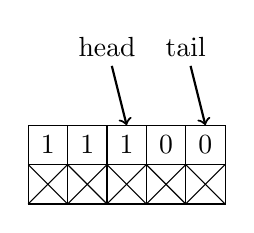
\begin{tikzpicture}
                \draw (0,0) rectangle (2.5,1);
                \draw (0,.5) -- (2.5,.5);
            \foreach \i in {.5,1,...,2}{
                \draw (\i,0) -- (\i,1);
            }
            \foreach \i/\j/\k in {0/1/0,1/1/0,2/1/1,3/0/0,4/0/0}{
                \node at (\i*.5+.25,.75) {\j};
                \ifthenelse{\k=1}{
                    \draw (\i*.5,0) -- (\i*.5+.5,.5);
                    \draw (\i*.5,.5) -- (\i*.5+.5,0);
                }{};
            }
            \node at (1,2) (b) {head};
            \node at (2,2) (e) {tail};
            \draw [thick,->] (b) -- (1.25,1);
            \draw [thick,->] (e) -- (2.25,1);

            \end{tikzpicture}
            \caption{Initial example}
            \label{fig:reorder0}
        \end{subfigure}
        \begin{subfigure}{.32\linewidth}
            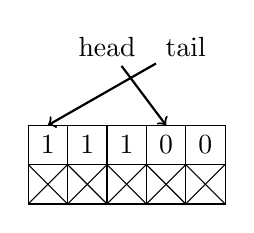
\begin{tikzpicture}
                \draw (0,0) rectangle (2.5,1);
                \draw (0,.5) -- (2.5,.5);
            \foreach \i in {.5,1,...,2}{
                \draw (\i,0) -- (\i,1);
            }
            \foreach \i/\j/\k in {0/1/0,1/1/0,2/1/0,3/0/0,4/0/0}{
                \node at (\i*.5+.25,.75) {\j};
                \ifthenelse{\k=1}{
                    \draw (\i*.5,0) -- (\i*.5+.5,.5);
                    \draw (\i*.5,.5) -- (\i*.5+.5,0);
                }{};
            }
            \node at (1,2) (b) {head};
            \node at (2,2) (e) {tail};
            \draw [thick,->] (b) -- (1.75,1);
            \draw [thick,->] (e) -- (.25,1);

            \end{tikzpicture}
            \caption{First clock cycle}
            \label{fig:reorder1}
        \end{subfigure}
        \begin{subfigure}{.32\linewidth}
            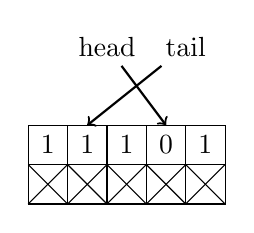
\begin{tikzpicture}
                \draw (0,0) rectangle (2.5,1);
                \draw (0,.5) -- (2.5,.5);
            \foreach \i in {.5,1,...,2}{
                \draw (\i,0) -- (\i,1);
            }
            \foreach \i/\j/\k in {0/1/0,1/1/0,2/1/0,3/0/0,4/1/1}{
                \node at (\i*.5+.25,.75) {\j};
                \ifthenelse{\k=1}{
                    \draw (\i*.5,0) -- (\i*.5+.5,.5);
                    \draw (\i*.5,.5) -- (\i*.5+.5,0);
                }{};
            }
            \node at (1,2) (b) {head};
            \node at (2,2) (e) {tail};
            \draw [thick,->] (b) -- (1.75,1);
            \draw [thick,->] (e) -- (.75,1);

            \end{tikzpicture}
            \caption{Second clock cycle}
            \label{fig:reorder2}
        \end{subfigure}
        \begin{subfigure}{.32\linewidth}
            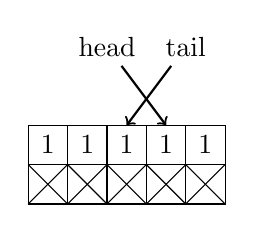
\begin{tikzpicture}
                \draw (0,0) rectangle (2.5,1);
                \draw (0,.5) -- (2.5,.5);
            \foreach \i in {.5,1,...,2}{
                \draw (\i,0) -- (\i,1);
            }
            \foreach \i/\j/\k in {0/1/0,1/1/0,2/1/0,3/1/1,4/1/1}{
                \node at (\i*.5+.25,.75) {\j};
                \ifthenelse{\k=1}{
                    \draw (\i*.5,0) -- (\i*.5+.5,.5);
                    \draw (\i*.5,.5) -- (\i*.5+.5,0);
                }{};
            }
            \node at (1,2) (b) {head};
            \node at (2,2) (e) {tail};
            \draw [thick,->] (b) -- (1.75,1);
            \draw [thick,->] (e) -- (1.25,1);

            \end{tikzpicture}
            \caption{Third clock cycle}
            \label{fig:reorder3}
        \end{subfigure}
        \begin{subfigure}{.32\linewidth}
            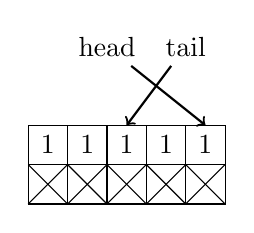
\begin{tikzpicture}
                \draw (0,0) rectangle (2.5,1);
                \draw (0,.5) -- (2.5,.5);
            \foreach \i in {.5,1,...,2}{
                \draw (\i,0) -- (\i,1);
            }
            \foreach \i/\j/\k in {0/1/0,1/1/0,2/1/0,3/1/0,4/1/1}{
                \node at (\i*.5+.25,.75) {\j};
                \ifthenelse{\k=1}{
                    \draw (\i*.5,0) -- (\i*.5+.5,.5);
                    \draw (\i*.5,.5) -- (\i*.5+.5,0);
                }{};
            }
            \node at (1,2) (b) {head};
            \node at (2,2) (e) {tail};
            \draw [thick,->] (b) -- (2.25,1);
            \draw [thick,->] (e) -- (1.25,1);

            \end{tikzpicture}
            \caption{Fourth clock cycle}
            \label{fig:reorder4}
        \end{subfigure}
        \begin{subfigure}{.32\linewidth}
            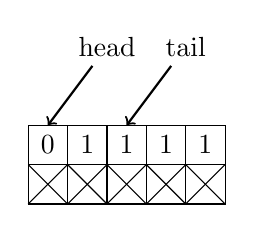
\begin{tikzpicture}
                \draw (0,0) rectangle (2.5,1);
                \draw (0,.5) -- (2.5,.5);
            \foreach \i in {.5,1,...,2}{
                \draw (\i,0) -- (\i,1);
            }
            \foreach \i/\j/\k in {0/0/1,1/1/0,2/1/0,3/1/0,4/1/0}{
                \node at (\i*.5+.25,.75) {\j};
                \ifthenelse{\k=1}{
                    \draw (\i*.5,0) -- (\i*.5+.5,.5);
                    \draw (\i*.5,.5) -- (\i*.5+.5,0);
                }{};
            }
            \node at (1,2) (b) {head};
            \node at (2,2) (e) {tail};
            \draw [thick,->] (b) -- (.25,1);
            \draw [thick,->] (e) -- (1.25,1);

            \end{tikzpicture}
            \caption{Fifth clock cycle}
            \label{fig:reorder5}
        \end{subfigure}
        %\input{fig/reorder.tex}
        \caption[The reorder queue]{Reorder queue example.}
        \label{fig:reorder}
    \end{figure}

    The buffering in both designs ensures relatively high throughput, however, this buffering causes a problem for both memories, as read responses from different banks from the same port may come back out of order. Although out of order reads do not always cause an issue, to alleviate this issue we add reorder queues to both multi-port memory designs.

    A reorder queue behaves similarly to a FIFO. However, some of the values in between the head and tail pointer exist ``in flight'' and not at the reorder queue memory. The reorder queue keeps track of the presence of messages with a bit array (a 1-bit wide RAM).

    \figurename~\ref{fig:reorder} shows an example with 5 clock cycles of operation. In the initial state (\figurename~\ref{fig:reorder0}), the reorder queue has one present message and one in flight message.

         On the first clock cycle (\figurename~\ref{fig:reorder1}), the present message at the head gets popped from the queue. A new message increments the tail, but the message remains in flight until it arrives at the reorder queue.

         On the second clock cycle (\figurename~\ref{fig:reorder2}), a new message arrives at the reorder queue, however, it does not arrive at the head of the queue so no message can get popped.

         On the third clock cycle (\figurename~\ref{fig:reorder3}), a message arrives at the head of the reorder queue.

         On the fourth clock cycle (\figurename~\ref{fig:reorder4}), this message at the head of the reorder queue gets popped. If the reorder queue did not exist, the message that appeared on clock cycle 2 would have reached the output first even though it was sent later.

         On the fifth clock cycle (\figurename~\ref{fig:reorder5}), a message arrives. However, the meaning of 1 or 0 in the 1-bit RAM switched after the pointers wrapped around the end of the RAM. Instead of 1 meaning present, 1 now means in flight. This semantic flipping allows the use of only one write port on the 1-bit RAM (instead of two if the bits flipped after popping a message), saving on memory-related resources. 

\section{Evaluation}
\label{sec:evaluation}
    We limit linked list FIFOs and reorder queues to a depth of 64. We limit the depth of the FIFOs in the fully-connected interconnect network to 32 since the number of FIFOs in it grows by $O(N^2)$.

    We used the ModelSim logic simulator to evaluate the performance of each configuration. The testbench used for evaluation consists of four benchmarks. Each benchmark tests the read performance of sequential, random, congested, or segregated memory access patterns.

    We calculate the throughput of a given benchmark by measuring the ratio of read requests to potential read requests. If no stalls occur, the throughput equals 100\%. We calculate the latency by measuring the number of clock cycles between the last read request and the last read response. 
\begin{table*}
    \center
    \caption{Analysis of the Omega multi-port memory design.}
    \label{tbl:resources}
\begin{threeparttable}
\begin{tabular}{|l|l|l|l|l|l|}
\hline
Ports & & 4 & 8 & 16 & 32 \\
Memory Space & &  16KB & 32KB & 64KB & 128KB \\
\hline
 & \multicolumn{5}{|c|}{Fully-connected Multi-port Memory}\\
\cline{1-6}
\multirow{4}{*}{\shortstack[l]{Resource\\Utilization\\Virtex 7\\ V2000T\tnote{2}}} & Registers & 4K & 14K & 50K & 190K \\
                                                                          & LUTs      & 5.7K & 18K & 61K & 241K \\
& BlockRAM  & 4 & 8 & 16 & 32 \\
 & Clock frequency & 345Mhz & 313Mhz & 256Mhz & 273Mhz \\
\hline
Sequential & Throughput & 100\% & 100\% & 100\% & 100\% \\
 & Latency \tnote{1} & 16 & 20 & 36 & 64 \\
Random & Throughput & 97\% & 93\% & 88\% & 72\% \\
 & Latency \tnote{1} & 66 & 65 & 85 & 97 \\
Congested & Throughput & 25\% & 13\% & 6\% & 3\% \\ 
 & Latency \tnote{1} & 105 & 230 & 490 & 1034 \\
Segregated & Throughput & 100\% & 100\% & 100\% & 100\% \\
 & Latency \tnote{1} & 16 & 24 & 34 & 63 \\
\hline
 & \multicolumn{5}{|c|}{Omega Multi-port Memory} \\
\hline
\multirow{4}{*}{\shortstack[l]{Resource\\Utilization\\Virtex 7\\ V2000T\tnote{2}}}& Registers & 3K & 9K & 22K & 53K \\
                                                                      & LUTs      & 5K & 11K & 24K & 53K \\
& BlockRAM  & 4 & 8 & 16 & 32 \\
& Clock frequency & 258Mhz & 257Mhz & 260Mhz & 262Mhz \\
\hline
Sequential & Throughput & 100\%  & 100\% & 100\% & 100\% \\
& Latency \tnote{1} & 17 & 25 & 37 & 56 \\
Random & Throughput & 94\% & 83\% & 68\% & 52\% \\
 & Latency \tnote{1} & 72 & 110 & 131 & 193 \\
Congested & Throughput & 25\% & 13\% & 6\% & 3\% \\
 & Latency \tnote{1} & 250 & 462 & 786 & 1046 \\
Segregated & Throughput & 25\% & 13\% & 6\% & 3\% \\
 & Latency \tnote{1} & 247 & 461 & 756 & 1043 \\
\hline
\end{tabular}
\begin{tablenotes}
\item[1] This measures the number of clock cycles between the end of the benchmark and when the last response of the last request gets received. In the worst case scenario several FIFOs queue data that has to wait for access to the same bank.
\item[2] This particular chip has 2.4M registers, 1.2M LUTs and 1.3K RAM blocks.
\end{tablenotes}
\end{threeparttable}
\end{table*}



\section{Results}
\label{sec:analysis}
\begin{figure}[t]
    \center
    \begin{tikzpicture}[xscale=.19,yscale=.07]
        \tikzstyle{blueSquare}=[draw, rectangle, fill=blue, inner sep =2.5pt];
        \tikzstyle{redCircle}=[draw, circle, fill=red, inner sep =2.1pt];
        \tikzstyle{greenDiamond}=[draw, diamond, fill=green, inner sep =1.8pt];
        \tikzstyle{blackTriangle}=[draw, regular polygon, regular polygon sides=3, fill=black, inner sep =1.6pt];
        \draw [->] (0,0) -- (40,0);
        \draw [->] (0,0) -- (0,100);
        \foreach \i in {4,8,16,32}{
            \draw (\i,1) -- (\i,-1)node[anchor=20,rotate=60]{\i};
        }
        \foreach \y in {20,40,...,80}{
            \FPeval{\v}{round(\y*2.5:0)};
            \draw (.4,\y) -- (-.4,\y)node[anchor=south,rotate=90]{\v K};
        }
        \node at (20, -10) {Ports};
        \node at (-4,50) [rotate=90]{LUTs/Registers};
\foreach \xa/\ya/\xb/\yb in {4/4.1/8/14.0,8/14.0/16/50.0,16/50.0/32/190.0}{
    \draw [thick, red] (\xa,\ya/2.5) -- (\xb,\yb/2.5);
}
\foreach \xa/\ya/\xb/\yb in {4/5.7/8/18.0,8/18.0/16/61.0,16/61.0/32/241.0}{
    \draw [thick, blue] (\xa,\ya/2.5) -- (\xb,\yb/2.5);
}
\foreach \xa/\ya/\xb/\yb in {4/3.1/8/8.5,8/8.5/16/22.1,16/22.1/32/52.7}{
    \draw [thick, black] (\xa,\ya/2.5) -- (\xb,\yb/2.5);
}
\foreach \xa/\ya/\xb/\yb in {4/4.9/8/10.9,8/10.9/16/24.0,16/24.0/32/53.0}{
    \draw [thick, green] (\xa,\ya/2.5) -- (\xb,\yb/2.5);
}
\foreach \x/\y/\a in {4/4.1/18,8/14.0/15,16/50.0/0,32/190.0/0}{
    \FPeval{\ys}{round(\y:0)}
    \node[redCircle] at (\x,\y/2.5) [label={[inner sep=0,xshift=3pt,red, fill=white, yshift=\a pt]0:\small \ys K}] {};
    %\node[draw,fill=red,circle,inner sep=1.5pt] at (\x,\y/2.5) [label={[inner sep=0,xshift=3pt,red, fill=white, yshift=\a pt]0:\small \ys K}] {};
}
\foreach \x/\y/\a in {4/5.7/25,8/18.0/20,16/61.0/0,32/241.0/0}{
    \FPeval{\ys}{round(\y:0)}
    \node[blueSquare] at (\x,\y/2.5) [label={[inner sep=0,xshift=3pt,blue, fill=white,yshift=\a pt]0:\small \ys K}] {};
    %\node[draw,fill=blue,inner sep=1.5pt] at (\x,\y/2.5) [label={[inner sep=0,xshift=3pt,blue, fill=white,yshift=\a pt]0:\small \ys K}] {};
}
\foreach \x/\y/\a in {4/3.1/0,8/8.5/0,16/22.1/0,32/52.7/0}{
    \FPeval{\ys}{round(\y:0)}
    %\node[draw,regular polygon, regular polygon sides=3,fill=black,inner sep=1.5pt] at (\x,\y/2.5) [label={[inner sep=0,xshift=3pt,black, fill=white,yshift=\a pt]0:\small \ys K}] {};
    \node[blackTriangle] at (\x,\y/2.5) [label={[inner sep=0,xshift=3pt,black, fill=white,yshift=\a pt]0:\small \ys K}] {};
}
\foreach \x/\y/\a in {4/4.9/8,8/10.9/8,16/24.0/8,32/53.0/8}{
    \FPeval{\ys}{round(\y:0)}
    \node[greenDiamond] at (\x,\y/2.5) [label={[inner sep=0,xshift=3pt,green, fill=white,yshift=\a pt]0:\small \ys K}] {};
    %\node[draw,diamond,fill=green,inner sep=1.5pt] at (\x,\y/2.5) [label={[inner sep=0,xshift=3pt,green, fill=white,yshift=\a pt]0:\small \ys K}] {};
}

        \node at (15,90) []{\shortstack[l]{\tikz \node[blueSquare] at (0,0) {}; Fully-connected LUTs\\
                                            \tikz \node[redCircle] at (0,0) {}; Fully-connected Registers\\
                                            \tikz \node[greenDiamond] at (0,0) {}; Omega LUTs\\
                                            \tikz \node[blackTriangle] at (0,0) {}; Omega Registers}};
    \end{tikzpicture}
    \caption[Graph showing the increase in resource utilization as the number of ports in the Omega memory increases.]{The effect of varying the number of ports on FPGA resource utilization (area). The Fully-connected memory grows by approximately $N^2$ and the Omega memory grows almost linearly.}
    \label{fig:portresources}
\end{figure}

\begin{figure}
    \center
    \begin{tikzpicture}[xscale=.19,yscale=.07]
        \tikzstyle{blueSquare}=[draw, rectangle, fill=blue, inner sep =2.5pt];
        \tikzstyle{redCircle}=[draw, circle, fill=red, inner sep =2.1pt];
        \tikzstyle{greenDiamond}=[draw, diamond, fill=green, inner sep =1.8pt];
        \tikzstyle{blackTriangle}=[draw, regular polygon, regular polygon sides=3, fill=black, inner sep =1.6pt];
        \draw [->] (0,0) -- (40,0);
        \draw (0,0) -- (0,100);
        \foreach \i in {4,8,16,32}{
            \draw (\i,1) -- (\i,-1)node[anchor=20,rotate=60]{\i};
        }
        \node at (20, -10) {Ports};
        \node at (-4,50) [rotate=90]{Throughput};
        \foreach \i in {20,40,...,100}{
            \draw (.4,\i) -- (-.4,\i) node[anchor=south,rotate=90]{\i\%};
        }
\foreach \xa/\ya/\xb/\yb in {4/96.5/8/93.5,8/93.5/16/87.7,16/87.7/32/72.0}{
    \draw [thick, blue] (\xa,\ya/1) -- (\xb,\yb/1);
}
\foreach \x/\y/\a in {4/96.5/0,8/93.5/0,16/87.7/0,32/72.0/0}{
    \FPeval{\ys}{round(\y:0)}
    \node[blueSquare] at (\x,\y/1) [label={[inner sep=0,xshift=3pt,blue, fill=white,yshift=\a pt]0:\small \ys \%}] {};
}
\foreach \xa/\ya/\xb/\yb in {4/94.0/8/82.9,8/82.9/16/68.2,16/68.2/32/51.7}{
    \draw [thick, green] (\xa,\ya/1) -- (\xb,\yb/1);
}
\foreach \x/\y/\a in {4/94.0/-10,8/82.9/0,16/68.2/0,32/51.7/0}{
    \FPeval{\ys}{round(\y:0)}
    \node[greenDiamond] at (\x,\y/1) [label={[inner sep=0,xshift=3pt,green, fill=white,yshift=\a pt]0:\small \ys \%}] {};
}
        \node at (15,20) []{\shortstack[l]{\tikz \node[blueSquare] at (0,0) {}; Fully-connected\\
        \tikz \node[greenDiamond] at (0,0) {}; Omega}};

    \end{tikzpicture}
    \caption[Graph showing the effect on throughput as the number of ports on the Omega memory increases.]{The effect of varying the number of ports on throughput of the random memory access benchmark on the small resource memories.}
    \label{fig:portthroughput}
\end{figure}

We present the results of the Omega memory in Table \ref{tbl:resources} and include results from a Fully-connected memory as a comparison.
\subsection{Varying the number of ports}
In terms of area, \figurename~\ref{fig:portresources} shows the effect on FPGA logic resources due to varying the number of ports. As expected, the Fully-connected memory consumes resources at a rate of approximately $O(N^2)$. The Omega memory consumes resources at a slower rate of approximately $O(NlogN)$. At 8 ports, the Fully-connected memory consumes 50\% more resources than the Omega memory.\par
In terms of performance, \figurename~\ref{fig:portthroughput} shows that increasing the number of ports decreases throughput, and Table~\ref{tbl:resources} shows increasing the number of ports increases latency. As expected, throughput decreases a little faster for the Omega memory. The latency grows almost linearly with the number of ports, because of the round robin contention resolution scheme. On average it takes $\frac{N}{2}$ clock cycles to start processing the first memory request.

\subsection{Varying the buffer depth} Increasing the buffer depth, i.e. the reorder queue depth and the linked list FIFO depth, increases the throughput of the memories. \figurename~\ref{fig:reorderthroughput} shows that the throughput increases by around $O(1-(\frac{p-1}{p})^N)$, where $p$ equals the number of ports and $N$ equals the buffer depth. $1-(\frac{p-1}{p})^N$ equals the probability that at least one of the last $N$ memory requests requested data on bank0 (or any specific bank). This approximately equals the probability that the next FIFO in the round robin has at least one message.

\begin{figure}
    \center
    \begin{tikzpicture}[xscale=.19,yscale=.07]
        \tikzstyle{blueSquare}=[draw, rectangle, fill=blue, inner sep =2.5pt];
        \tikzstyle{redCircle}=[draw, circle, fill=red, inner sep =2.1pt];
        \tikzstyle{greenDiamond}=[draw, diamond, fill=green, inner sep =1.8pt];
        \tikzstyle{blackTriangle}=[draw, regular polygon, regular polygon sides=3, fill=black, inner sep =1.6pt];
        \draw [->] (0,0) -- (40,0);
        \draw (0,0) -- (0,100);
        \foreach \i in {4,8,16,32}{
            \FPeval{\r}{round(\i*4:0)}
            \draw (\i,1) -- (\i,-1)node[anchor=20,rotate=60]{\r};
        }
        \node at (20, -15) {Reorder Queue and Linked List FIFO Depth};
        \node at (-4,50) [rotate=90]{Throughput};
        \foreach \i in {20,40,...,100}{
            \draw (.4,\i) -- (-.4,\i) node[anchor=south,rotate=90]{\i\%};
        }
\foreach \xa/\ya/\xb/\yb in {4/64.0/8/84.0,8/84.0/16/93.4,16/93.4/32/97.2}{
    \draw [thick, blue] (\xa,\ya/1) -- (\xb,\yb/1);
}

\foreach \xa/\ya/\xb/\yb in {4/50.8/8/69.5,8/69.5/16/82.9,16/82.9/32/91.6}{
    \draw [thick, green] (\xa,\ya/1) -- (\xb,\yb/1);
}
\foreach \x/\y/\a in {4/50.8/0,8/69.5/0,16/82.9/0,32/91.6/0}{
    \FPeval{\ys}{round(\y:0)}
    \node[greenDiamond] at (\x,\y/1) [label={[inner sep=0,xshift=3pt,green, fill=white,yshift=\a pt]0:\small \ys \%}] {};
}
\foreach \x/\y/\a in {4/64.0/0,8/84.0/0,16/93.4/0,32/97.2/0}{
    \FPeval{\ys}{round(\y:0)}
    \node[blueSquare] at (\x,\y/1) [label={[inner sep=0,xshift=3pt,blue, fill=white,yshift=\a pt]0:\small \ys \%}] {};
}
        \node at (30,20) []{\shortstack[l]{\tikz \node[blueSquare] at (0,0) {}; Fully-connected\\
        \tikz \node[greenDiamond] at (0,0) {}; Omega}};
    \end{tikzpicture}
    \caption[Graph showing the increase in throughput as buffer depth increases.]{The effect of varying the depth of the linked list FIFOs and reorder queues on throughput of the random memory access benchmark (using 8-port memories).}
    \label{fig:reorderthroughput}
\end{figure}

\begin{figure}
    \center
    \begin{tikzpicture}[xscale=.19,yscale=.07]
        \tikzstyle{blueSquare}=[draw, rectangle, fill=blue, inner sep =2.5pt];
        \tikzstyle{redCircle}=[draw, circle, fill=red, inner sep =2.1pt];
        \tikzstyle{greenDiamond}=[draw, diamond, fill=green, inner sep =1.8pt];
        \tikzstyle{blackTriangle}=[draw, regular polygon, regular polygon sides=3, fill=black, inner sep =1.6pt];
        \draw [->] (0,0) -- (40,0);
        \draw [->] (0,0) -- (0,100);
        \foreach \i in {4,8,16,32}{
            \FPeval{\w}{round(\i*4:0)}
            \draw (\i,1) -- (\i,-1)node[anchor=20,rotate=60]{\w};
        }
        \foreach \y in {20,40,...,80}{
            \FPeval{\v}{round(\y*.3:0)};
            \draw (.4,\y) -- (-.4,\y)node[anchor=south,rotate=90]{\v K};
        }
        \node at (20, -10) {Width};
        \node at (-4,50) [rotate=90]{LUTs/Registers};
\foreach \xa/\ya/\xb/\yb in {4/8.3/8/11.7,8/11.7/16/18.1,16/18.1/32/30.5}{
    \draw [thick, blue] (\xa,\ya/.3) -- (\xb,\yb/.3);
}
\foreach \x/\y/\a in {4/8.3/0,8/11.7/0,16/18.1/0,32/30.5/0}{
    \FPeval{\ys}{round(\y:0)}
    \node[blueSquare] at (\x,\y/.3) [label={[inner sep=0,xshift=3pt,blue, fill=white,yshift=\a pt]0:\small \ys K}] {};
}
\foreach \xa/\ya/\xb/\yb in {4/6.0/8/8.7,8/8.7/16/13.9,16/13.9/32/24.6}{
    \draw [thick, red] (\xa,\ya/.3) -- (\xb,\yb/.3);
}
\foreach \x/\y/\a in {4/6.0/0,8/8.7/0,16/13.9/0,32/24.6/0}{
    \FPeval{\ys}{round(\y:0)}
    \node[redCircle] at (\x,\y/.3) [label={[inner sep=0,xshift=3pt,red, fill=white,yshift=\a pt]0:\small \ys K}] {};
}
\foreach \xa/\ya/\xb/\yb in {4/3.3/8/6.6,8/6.6/16/10.9,16/10.9/32/18.6}{
    \draw [thick, green] (\xa,\ya/.3) -- (\xb,\yb/.3);
}
\foreach \xa/\ya/\xb/\yb in {4/3.1/8/5.0,8/5.0/16/8.5,16/8.5/32/16.7}{
    \draw [thick, black] (\xa,\ya/.3) -- (\xb,\yb/.3);
}
\foreach \x/\y/\a in {4/3.1/0,8/5.0/0,16/8.5/0,32/16.7/0}{
    \FPeval{\ys}{round(\y:0)}
    \node[blackTriangle] at (\x,\y/.3) [label={[inner sep=0,xshift=3pt,black, fill=white,yshift=\a pt]0:\small \ys K}] {};
}
\foreach \x/\y/\a in {4/3.3/8,8/6.6/0,16/10.9/0,32/18.6/0}{
    \FPeval{\ys}{round(\y:0)}
    \node[greenDiamond] at (\x,\y/.3) [label={[inner sep=0,xshift=3pt,green, fill=white,yshift=\a pt]0:\small \ys K}] {};
}
        \node at (15,90) []{\shortstack[l]{\tikz \node[blueSquare] at (0,0) {}; Fully-connected LUTs\\
                                            \tikz \node[redCircle] at (0,0) {}; Fully-connected Registers\\
                                            \tikz \node[greenDiamond] at (0,0) {}; Omega LUTs\\
                                            \tikz \node[blackTriangle] at (0,0) {}; Omega Registers}};
    \end{tikzpicture}
    \caption[Graph showing the increase in resource utilization as the bit-width of the memory increases.]{The effect of varying the bit-width of the memory on FPGA resource utilization.}
    \label{fig:width}
\end{figure}

Increasing the buffer depth increases the latency. The buffers fill up over time as they attempt to prevent the memory from stalling. Full buffers means latency increases by the depth of the buffer. So in benchmarks with contention, the latency increases linearly with the buffer depth.

Increasing the buffer depth increases FPGA utilization. The increase in buffer depth affects the Omega memory more since the Fully-connected memory does not have linked list FIFOs. If we use RAM blocks for buffers, any depth less than 512 results in using approximately the same number of resources. But, if buffers consist entirely of distributed RAMs (LUT resources), FPGA utilization increases linearly with the buffer depth.

\subsection{Varying the data bit width} Data width only effects resource utilization. As \figurename~\ref{fig:width} shows, FPGA utilization scales linearly with the data bit width. However, bit width does effect throughput when measuring by bytes per second instead of by percentage. The bytes per second measurement equals $PERCENT\_THROUGHPUT \times PORT\_COUNT \times BIT\_WIDTH \times CLOCK\_FREQUENCY$. For example, the throughput on the random benchmark of the Omega memory with 16 ports is 35 GB/s.
